\documentclass[12pt]{article}

\title{Exploring the Presidents Corpus}

\author{
	Jomar Alcantara \\
	Department of Computer Science\\
	School of Engineering and Applied Sciences\\
	Aston University\\
	\texttt{alcantaj@aston.ac.uk} \\
		\and
	\textbf{Peter Sawyer} \\
	Department of Computer Science\\
	School of Engineering and Applied Sciences\\
	Aston University\\
	\texttt{p.sawyer@aston.ac.uk} \\
		\AND
	George Vogiatzis\\
	Department of Computer Science\\
	School of Engineering and Applied Sciences\\
	Aston University \\
	\texttt{g.vogiatzis@aston.ac.uk} \\
		\and
	\textbf{Felipe Campelo Franca Pinto}\\
	Department of Computer Science\\
	School of Engineering and Applied Sciences\\
	Aston University\\
	\texttt{f.campelo@aston.ac.uk}
}
	
\date{\today}

\usepackage{arxiv}
\usepackage{float}
\usepackage{graphicx}

\begin{document}
\maketitle

\keywords{Mild Cognitive Impairment \and Alzheimer's Disease \and Machine Learning \and Diagnosis \and Natural Language Processing} 
\bigskip
\begin{abstract}
This is the paper's abstract \ldots
\end{abstract}

\section{Introduction}\label{introduction}
The diagnosis of dementia is generally made when there is a decline in brain function due to physical changes in the brain \cite{Albert2011}. It affects a significant proportion of the global older adult population and the impact on morbidity and mortality rates is considerable. Dementia is currently the leading cause of death in England and Wales and the sixth leading cause of death in the United States (US). A 2014 report commissioned by the Alzheimer's Society estimated that in the UK by 2015 there would be approximately 855,000 people rising living with dementia increasing to 1 million by 2021 \cite{}. This represents 1 in 79 of the total UK population rising to 1 in 14 of those aged 65 or over \cite{AlzheimersSociety2014}. Worldwide, there are 46 million people with a diagnosis of dementia globally and that number is expected to hit 131.5 million by 2050 \cite{Prince2015}. From a financial perspective, the cost burden is also significant. The estimated annual spend on dementia healthcare in the UK is £4.3 billion of which approximately £85 million is spent on diagnosis. The total financial burden of dementia (excluding the costs associated with early onset dementia) is £26.3 billion annually. Globally, this picture is a lot bleaker. The worldwide cost of dementia in 2018 was estimated to be in the region of one trillon US dollars \cite{}.
\par 
There are different types of dementia including Alzheimer's Disease (AD), vascular dementia, dementia with Lewy bodies and fronto-temporal dementia, all of which are currently incurable. AD is a progressive neurodegenerative disease and is the most common type of dementia, responsible for approximately XX\% of all cases \cite{}. Currently, a definitive diagnosis for AD can only be produced at post-mortem. However, there are a number of psychological and physiological indicators that can indicate that dementia is present. From a physiological perspective, researchers have identified two proteins called beta-amyloid and tau have been identified as two of the key proteins that have a role in initiation and progression of AD. In a typical case beta-amyloid clumps into plaques which slowly build up between neurons with tau proteins accumulating and eventually forming tangles inside neurons. At a certain point, the levels of beta-amyloid rise triggering a more rapid spread of tau throughout the brain. Eventually, due to these and other changes, neurons lose their ability to communicate and the brain starts to shrink. This leads to the development of some of the psychological symptoms associated with AD, primarily cognitive deficits such as problems with episodic and semantic memory, organizing and planning, difficulties with language, problems with executive function and visuospatial deficits \cite{McKhann2011}. These cognitive symptoms are often accompanied by emotional problems such as depression and behavioural difficulties. As more neurons die throughout the brain, a person with AD gradually loses the ability to think, remember, make decisions and function independently.
\par
Despite the increasing prevalence of AD and an improved understanding about how it affects the brain there are no medications that improve prognosis. All the medications that are currently on the market are designed to manage symptoms. Whilst there are numerous investigational drugs in development for the treatment of AD, a larger than normal percentage of these drugs fail in clinical trial stage of the drug discovery process ((99.6\% failure rate vs 80\% for systemic anti-cancer drugs) \cite{Cummings2014}. Cummings et al proposed that a possible reason for the lack of success is that the drugs treatments are initiated too far along in the progression of the disease and thus much of the degeneration of the brain has already occurred \cite{Cummings2014}. Research focus has now started to shift to the earlier stages of AD (i.e. symptomatic pre-dementia phase of AD) which some literature describes as 'Mild Cognitive Impairment (MCI) due to AD'.
\par
One of the challenges associated with the early detection of AD is differentiating natural age associated memory impairment and cognitive decline due to aging from with decline due to AD. This challenge is often complicated further due to the large variation in the cognitive abilities and educational background of individuals. The work of Albert et al helps to address this by the development of clinical criteria which professionals can use to diagnose MCI due to AD. One of the most important observations from this piece of work is that a diagnosis of MCI requires evidence of intra-individual change and optimally requires evaluation at two or more points \cite{Albert2011}, and this is essentially to place more importance on the trajectory of a person's cognitive abilities rather than a person's cognitive ability in general. 
\par 
There has been a significant research in the area of language deterioration as a method of detecting AD at an earlier stage. This usually takes the form of recording speech whilst patients' undertake a cognitive assessment such as the Picture Description Task \cite{Orimaye2014,Fraser2015}. Given that language samples are relatively easy to collect, research has moved towards analysis of spontaneous speech. The work of Berisha and Liss is a good example of this, this study compared the differences in language use between two US presidents, Ronald Reagan (RR), who would go on to receive a diagnosis of Dementia and George H. W. Bush (GHWB) who acted as a matched control based on Age \cite{Berisha2015}. They found several differences in language use over time which they felt acted as indicators of RR's difficulties with language due to AD. Differences in features of language identified to be statistically significant included the number of unique words used per speech, the use of non-specific nouns and fillers and low imageability verbs \cite{Berisha2015}. 
\par   
This study replicates the research of Berisha and Liss and extends this by adding Donald Trump (DJT) as an additional comparison to RR. This study aims to contribute to our understanding of the pre-diagnosis phase of Alzheimer's Disease and it's effect on language. Our hypothesis is that there will be features of RR's language which change more noticably over time when compared with the two closest appropriate controls. Compared to the previous research study, we explored a wider range of language features within this dataset. In addition, our assumption was that any language deterioration found would be non-linear and so we will be looking at non linear and linear correlations within the data were looked at to see if language decline is constant over time

\section{Methodology}\label{methodology}
We took 46 transcripts of press conferences given by RR (from 1981 to 1988) and compared them with 134 press conferences (from 1989 to 1993) given by GHWB and 29 press conferences (from 2016 to 2019) conducted by DJT.  We analysed transcripts for language features (described below) shown to change longitudinally with AD. These language features are analysed at the word level, sentence level and document level. 
\par 
In the original study, GHWB was selected as the comparator president as he was the closest match in terms of age to RR (GHWB - age at the start of presidency: 64 years and 222 days vs RR: 69 years and 349 days). However, since his inauguration, DJT is now the closest comparible president in terms of age (DJT - age at the start of presidency: 70 years and 220 days). We included DJT who like GHWB has no known diagnosis of AD to determine whether the comparisons made by Berisha and Liss hold true with this closer presidential match in terms of age. 
\par 
We used the press conference transcripts in the American Presidency Project (APP) archive as a data source for this project. The APP is a comprehensive and organized searchable database of presidential documents, including transcripts of speeches, transcripts of news conferences, and other public documents. These documents are open access and can be downloaded at any time from the APP archive.

\subsection{Pre-processing}
To generate the files necessary for analysis, we downloaded each transcript and performed the following changes. We omitted the prepared statement by the president and any speech by other individuals and started each transcript at the beginning of the first answer to a question by a member of the press. We filtered any annotations that were added to the transcript, including any references or clarifications, and any laughter. It's worth noting that there appears to be a difference in how 'hesitations' were marked down between each president, for RR \& DJT hesitations were marked by a single hyphen whereas for GHWB hesitations are marked by a double hyphen. In order to maintain consistency when parsing through the documents, We have changed both types of hesitation to be marked by a single hyphen. We also omitted one word sentences as this data would, from a theoretical perspective, not be relevant for language analysis. We did not control for the length of the document, but generated features which would normalise by the length of the document. We therefore was able to include all press conferences by all presidents analysed where there was a question and answer session conducted at least in part by the president in question (2 press conferences of GHWB were omitted due to a lack of a question and answer session).

\subsection{Feature Generation}
We calculated the following features for each transcript in turn using the Natural Language ToolKit (NLTK) package \cite{Bird2009}, Linguistic Inquiry and Word Count (LIWC) \cite{Pennebaker2015} and Python. Words were stemmed to their root form using the Porter2 (Snowball) stemmer algorithm. 
\par 
\subsubsection{Measures of lexical diversity}
Lexical diversity is a measure of the variety of language used within a given document. A document is said to have high lexical diversity if the number of unique words is large. We constructed four features of lexical variation. Firstly we looked at the number of unique words. To do this we were able to split each transcript into individual words and changed them to lowercase using NLTK and were then count the number of unique words that appeared in each transcript. We also used the TTR formula, Brunet's Index and Honore's Statistic as other measures of lexical diversity \cite{Richards1987}. 
\par 
Type token ratio (TTR) is the ratio obtained by dividing the types (The total number of different words) by the tokens (the total number of words in an utterance).
\begin{equation} \label{x1}
TTR = numberOfUniqueWords / totalNumberOfWords.
\end{equation}
\par 
Brunet's Index (W) differentiates itself from TTR, as it is not impacted by the length of the text itself. Brunet's Index is defined by the following equation:
\begin{equation} \label{x2}
W = N^{V(-0.165)}
\end{equation}
where N is the total length of the utterance being measured and V is equal to the total vocabulary being used by the subject. Brunet's Index usually has a score of between 10 and 20, with high numbers indicating a more rich vocabulary compared to low numbers. \newline
\par 
Honore's Statistic is based on the idea that vocabulary richness is implied when a speaker uses a greater amount of unique words. This is indicated by the following equation: 
\begin{equation} \label{x3}
%% Check to see if this is accurate.
R = (100 \log N) / (1 - V1/V)
\end{equation}
where v1 is equal to the number of unique words, V is the total vocabulary used and N is the total number of words in the utterance being measured.
\subsubsection{Fillers, Non-Specific Nouns and Low Imageability Verbs}
Fillers, Non-Specific Nouns and Low Imageability Verbs were features used by Berisha and Liss in their research \cite{Berisha2015} and were taken from work done by Bird et al \cite{Bird2000}. Fillers can be described as a potentially meaningless word that marks a pause or hesitation in speech. In those with MCI and AD, these words can be used to temporarily disguise problems in thought processes or word finding difficulties. Non-Specific Nouns refer to a category or an unspecified member of a given category, once again this can be characterised as a compensatory strategy for word finding difficulties. Imageability is characterized, according to Berisha and Liss, as the ease with which a word provokes a mental image of what the word describes. 

\begin{table}[H]
	\begin{center}
	\begin{tabular}{ | p{3cm} | p{10cm} |}
		\hline
		Category & Words \\ \hline
		Fillers & \textit{"um", "uh", "er", "ah", "like", "okay", "right",  "you know", "well", "so", "basically", "actually", "literally"} \\ \hline
		Non Specific Nouns & \textit{"something", "anything", "thing", "everything"} \\ \hline
		LI Verbs & \textit{"be", "come", "do", "get", "give", go", "know", "look", "make", "see", "tell", "think", "want"} \\ \hline
	\end{tabular}
	\caption{\label{tab:table-name}Examples of words belonging to the categories Fillers, Non-Specific Nouns and Low Imageability Verbs}
	\end{center} 
\end{table}

\subsubsection{Usage of parts of speech}
Using a Part of Speech tagger (PoS) on each transcript analyses each sentence within the transcript and assigns a 'tag' to each word based on the function the word has in a sentence. At a basic level this can be divided into the eight defined parts of speech: 'nouns', 'pronouns', verbs', 'adjectives', 'adverbs', 'conjunctions', 'prepositions' and 'interjections' but can be further subcategorised. We used the PoS tagger built into NLTK to tag each transcript in turn and used these the counts from each of these eight categories in our analysis. In addition to frequency counts we also normalised these features by dividing the frequency count by the number of words in the document to take into account transcript length.

\subsubsection{Linguistic Inquiry and Word Count(LIWC)}
The LIWC is a text processor which analysis words within a given a document and compares the words in the LIWC dictionary file. The LIWC dictionary file contains over 6000 words which are categorised into approximately 90 different types. For example the word 'cried' is part of five word categories: sadness, negative emotion, overall affect, verbs and past focus \cite{Pennebaker2015}. Each word in the document or set of documents is searched for in the dictionary file and if found, the appropriate type is incremented by 1. What is output is an analysis of word usage in reference to each category. This is particularly useful in analysing both structural language changes but also the content or themes of language for a given transcript or set of transcripts.
\par 
As with Berisha and Liss, we analysed the transcripts over time in order to determine if there was an underlying temporal trend that may indicate that different parts of language increase or decrease over time. In AD, cognitive abilities are said to deteriorate over time and therefore it may be useful to analyse temporal trends that indicate a potential deterioration of cognition. In order to get a accurate measure of deterioration over time, we time stamped each transcript in relation to number of days from the first transcript to the date of the transcript being analysed as the press conferences were not evenly spaced out during the presidencies.

\section{Results}\label{results}
One of the most important thing to note is the wide variety of samples between the three presidents and also the varying timescales. RR participated in 46 press conferences over eight years (an average of 5.75 a year) which is the fewest number of press conferences given by an American president during their term of office. GHWB participated in 136 press conferences over four years (an average of 34 a year) and DJT participated in 29 press conferences to date (an average of 19.3 per year). Equally, there are differences in the average number of words. RR produced an average of 3424 words per conference compared to 2608 by GHWB (unpaired t = 4.434, p\textless 0.001) and DJT at 1849 words (unpaired t = 6.524, p\textless 0.001).

\begin{table}[H]
	\begin{center}
	\begin{tabular}{ | p{3cm} | p{1.5cm} | p{1.5cm} | p{1.5cm} |}
		\hline
		& RR & GHWB & DJT \\ \hline
		Total Words & 3423.91 (416.42) & 2607.72 (1210.38) & 1848.65 (1549.38) \\ \hline
		Unique Words & 894.13 (85.15) & 667.76 (218.67) & 481.82 (221.29) \\ \hline
		Mean Length of Utterance & 23.17 (1.402) & 18.71 (2.067) & 13.84 (1.619) \\ \hline
	\end{tabular}
	\caption{\label{tab:table-name}Means and Standard Deviations of general features for each set of transcripts}
	\end{center} 
\end{table}

In terms of more specific language differences between the presidents, we found that RR used significantly more unique words, non-specific nouns and low imageability verbs than GHWB and DJT (see Table 3.3). The mean length of utterance for RR was significantly greater than that of GHWB and DJT. Some of these differences are due to the length of the sample, particularly in the case of DJT where his average sample is almost half the sample of RR. It could also be said that this could be down to differences in linguistic abilities or speaking style \cite{Berisha2015, Le2011}. However, we can certainly see that as controls GWHB and DJT are comparative in relation to non-specific nouns and LI verbs. 

\begin{table}[H]
	\begin{center}
	\begin{tabular}{ | p{3cm} | p{1.5cm} | p{1.5cm} | p{1.5cm} |}
		\hline
		& RR v GHWB & RR v DJT & GHWB v DJT \\ \hline
		Total Words & \textbf{4.434***} & \textbf{6.524***} & \textbf{2.899**} \\ \hline
		Unique Stems & \textbf{10.878***} & \textbf{10.111***} & \textbf{4.148***} \\ \hline
		Mean Length of Utterance & \textbf{16.175***} & \textbf{25.084***} & \textbf{13.484***} \\ \hline	
		Non Specific Nouns & \textbf{7.877***} & \textbf{3.426**} & -0.574 \\ \hline
		LI Verbs & \textbf{2.656**} & \textbf{3.420***} & 1.628 \\ \hline
		\multicolumn{4}{@{}p{1.5in}}{\footnotesize * denotes p\textless 0.05} \\
		\multicolumn{4}{@{}p{1.5in}}{\footnotesize ** denotes p\textless 0.01} \\
		\multicolumn{4}{@{}p{1.5in}}{\footnotesize *** denotes p\textless 0.001} \\
	\end{tabular}
	\caption{\label{tab:table-name}RR T-tests vs GWB and DJT}
	\end{center} 
\end{table}

\subsection{Longitudinal Analysis}
We then looked at the data from a longitudinal perspective as we are interested seeing whether we can track various language variables and their progress over time. We ran a number of Pearsons correlations with transcript index number as a time reference and the dependant variables (Table 3.4).  For our controls, we found them to be stable for the most part with the main highlights being a decrease in Adverb usage for DJT (R=-0.36, p=0.049) and a steady but not severe decline in a number of variables for GWHB, namely total word count, unique words, low imageability words and verb usage.
\par 
For RR, his decline is more marked and more widespread through his language use. We noticed an significant increase in adverb (R=0.41, p=0.004) and pronoun usage (R=0.65, p\textless0.001), as well as a slight usage increase in Non-specific nouns(R=0.30, p=0.03). There was a highly significant decrease in number of unique words (R=-0.56, p\textless0.001) and noun usage (R=-0.70, p\textless0.001). Also very significant decrease in adjective usage (R=-0.40, p=0.005) and a significant decrease in total word count (R=-0.31, p=0.03). 

\begin{table}[H]
	\begin{center}
	\begin{tabular}{ | l | p{1.5cm} | p{1.5cm} | p{1.5cm} |}
		\hline
		& RR & GHWB & DJT \\ \hline
		Word Count & \textbf{-0.31*} & \textbf{-0.21*} & 0.08 \\ \hline 
		Unique Words & \textbf{-0.56***} & \textbf{-0.25**} & 0.16 \\ \hline
		Non Specific Nouns & \textbf{0.30*} & -0.08 & -0.03 \\ \hline
		LI Verbs & -0.19 & \textbf{-0.20**} & 0.02 \\ \hline
		Nouns Normalised & \textbf{-0.70***} & -0.03 & 0.14 \\ \hline
		Verbs Normalised & \textbf{0.36**} & \textbf{0.24***} & -0.03 \\ \hline
		Adjectives Normalised & \textbf{-0.40**} & 0.08 & -0.34 \\ \hline
		Adverbs Normalised & \textbf{0.41***} & 0.02 & \textbf{-0.36*} \\ \hline
		Pronouns Normalised & \textbf{0.65***} & 0.13 & 0.07 \\ \hline
		\multicolumn{4}{@{}p{1.5in}}{\footnotesize * denotes p\textless 0.05} \\
    	\multicolumn{4}{@{}p{1.5in}}{\footnotesize ** denotes p\textless 0.01} \\
    	\multicolumn{4}{@{}p{1.5in}}{\footnotesize *** denotes p\textless 0.001} \\
	\end{tabular}
	\caption{\label{tab:table-name}Pearson Correlations for Features}
	\end{center} 
\end{table}

Given the number of hypotheses being tested, it is necessary to apply some correction for family wise error rate and therefore a Hochberg step-up procedure was applied to the results of the analysis. We also used the Benjamini-Yekutieli procedure for controlling for False Discovery rate and came up with a final list of important features for each president. For RR, this was 22 features, for GHWB this was 14 features and there were no significant features for DJT after applying these methods.  The features were generated from multiple sources and therefore there was some significant overlap between the features. In these cases, the normalised features were prefered to raw count features. Where there was doubt as to the most appropriate feature, all features have been included. 

\begin{table}[H]
	\begin{center}
	\begin{tabular}{ | l | p{2.5cm} | p{2.5cm} | p{2.5cm} |}
		\hline
		& RR R-Squared  & GWB R-Squared & DJT R-Squared \\ \hline
		ppron & \textbf{0.700***} & 0.2 & 0.35 \\ \hline
		social & \textbf{0.698***} & 0.2 & 0.35 \\ \hline
		NounsNormalised & \textbf{-0.689***} & 0.2 & 0.35 \\ \hline
		function & \textbf{0.670***} & 0.2 & 0.35 \\ \hline
		conj &\textbf{0.644***} & 0.2 & 0.35 \\ \hline
		PronounsNormalised & \textbf{0.631***} & 0.2 & 0.35 \\ \hline
		Analytic & \textbf{-0.626***} & 0.2 & 0.35 \\ \hline
		NN & \textbf{-0.601***} & 0.2 & 0.35 \\ \hline
		male & \textbf{0.585***} & 0.2 & 0.35 \\ \hline
		UniqueWords & \textbf{-0.578***} & 0.2 & 0.35 \\ \hline
		WDT & \textbf{-0.577***} & 0.2 & 0.35 \\ \hline
		shehe & \textbf{0.529*} & 0.2 & 0.35 \\ \hline
		VBZ & \textbf{-0.521*} & 0.2 & 0.35 \\ \hline
		JJ & \textbf{-0.518*} & 0.2 & 0.35 \\ \hline
		Fillers & \textbf{-0.518*} & \textbf{-0.518*}  & 0.35 \\ \hline	
		EX & \textbf{-0.518*} & \textbf{-0.518*}  & 0.35 \\ \hline	
		achieve & \textbf{-0.518*} & \textbf{-0.518*}  & 0.35 \\ \hline		
		\multicolumn{4}{@{}p{1.5in}}{\footnotesize * denotes p\textless 0.05} \\
    	\multicolumn{4}{@{}p{1.5in}}{\footnotesize ** denotes p\textless 0.01} \\
    	\multicolumn{4}{@{}p{1.5in}}{\footnotesize *** denotes p\textless 0.001} \\

	\end{tabular}
	\caption{\label{tab:table-name}Pearson Correlations for Features}
	\end{center} 
\end{table}



\begin{table}[H]
	\begin{center}
	\begin{tabular}{ | l | p{2.5cm} | p{2.5cm} | p{2.5cm} |}
		\hline
		& RR R-Squared  & GWB R-Squared & DJT R-Squared \\ \hline
		ppron & \textbf{0.700***} & 0.2 & 0.35 \\ \hline
		social & \textbf{0.698***} & 0.2 & 0.35 \\ \hline
		NounsNormalised & \textbf{-0.689***} & 0.2 & 0.35 \\ \hline
		function & \textbf{0.670***} & 0.2 & 0.35 \\ \hline
		conj &\textbf{0.644***} & 0.2 & 0.35 \\ \hline
		PronounsNormalised & \textbf{0.631***} & 0.2 & 0.35 \\ \hline
		Analytic & \textbf{-0.626***} & 0.2 & 0.35 \\ \hline
		NN & \textbf{-0.601***} & 0.2 & 0.35 \\ \hline
		male & \textbf{0.585***} & 0.2 & 0.35 \\ \hline
		UniqueWords & \textbf{-0.578***} & 0.2 & 0.35 \\ \hline
		WDT & \textbf{-0.577***} & 0.2 & 0.35 \\ \hline
		shehe & \textbf{0.529*} & 0.2 & 0.35 \\ \hline
		VBZ & \textbf{-0.521*} & 0.2 & 0.35 \\ \hline
		JJ & \textbf{-0.518*} & 0.2 & 0.35 \\ \hline
		Fillers & \textbf{-0.518*} & \textbf{-0.518*}  & 0.35 \\ \hline	
		EX & \textbf{-0.518*} & \textbf{-0.518*}  & 0.35 \\ \hline	
		achieve & \textbf{-0.518*} & \textbf{-0.518*}  & 0.35 \\ \hline		
		\multicolumn{4}{@{}p{1.5in}}{\footnotesize * denotes p\textless 0.05} \\
    	\multicolumn{4}{@{}p{1.5in}}{\footnotesize ** denotes p\textless 0.01} \\
    	\multicolumn{4}{@{}p{1.5in}}{\footnotesize *** denotes p\textless 0.001} \\

	\end{tabular}
	\caption{\label{tab:table-name}Pearson Correlations for Features}
	\end{center} 
\end{table}


\section{Discussion}\label{discussion}
President Reagan received his diagnosis of AD in August 1994 but using transcripts of speeches he made in his two terms as President (January 1981 - January 1989) we have be able to identify certain changes in his use of language that we might ascribe to the onset of MCI and early AD. Despite differences in our methodology, our research supports some of the findings of Berisha and Liss in that we find an increase in non-specifc noun usage. Compared to our controls (GWHB and DJT), we find some slight trends with GWHB but no such trends with DJT in his speech albeit his samples of speech span a shorter amount of time.
\par 
A criticism of Berisha and Liss's work is the problems they had with normalising the transcripts in terms of length. This was also a problem in the work of Garrard et al \cite{Garrard2005, Le2011}. Whilst it is important to control for outliers, there are other ways in which we can control for length of sample. In this paper, we controlled for transcript length by dividing any features that were raw counts by the total length of the transcript. Given the increased amounts of hypothesis testing, it became necessary to control for false discoveries. 
\par 
Interestingly, when we normalised the various types of words used by the presidents we found some interesting patterns that further differentiated RR from the controls. Whilst Non-specific nouns increased over time, we found that noun usage in general significantly decreased and pronouns increased similarly significantly. The increase in pronoun for those with early AD has been identified in literature, although there are only a few studies that explore this \cite{Almor1999, Wendelstein2015}. Wendlestein et al propose that the increased used of pronouns is an expression of an impaired ability to adapt language to the listener's needs \cite{Wendelstein2015}. Almor et al attributed this reliance on pronouns due to a impaired working memory \cite{Almor1999}.
\par 
The decrease in overall noun usage has also been identified as a feature. Jarrold et al found that AD patients would use more pronouns, verbs and fewer nouns than controls \cite{Jarrold2014}. Wendlestein in their investigations into noun usage found that decreased later on in AD progression and was unaffected in the pre-clinical stages of AD \cite{Wendelstein2014}. Our results are supported by existing literature and this potentially means that language analysis in the way we have structured it may have diagnostic or prognostic properties.
One of the most striking differences between this study and the original is when looking at Unique Words. Whilst Unique Words as a feature is significant, which was a finding in the original study, when we controlled via normalisation, we found that this was not significant. 
\par
Another observation is that when conducting fitting a linear model to this data does not tell the whole story. For example, consider the following two plots. One shows a model fit to a linear  model, and the other shows a model fit using local polynomial regression model which aims to model the data more closely. 

\begin{figure}[b]
	\centering
	\begin{minipage}[b]{0.4\textwidth}
		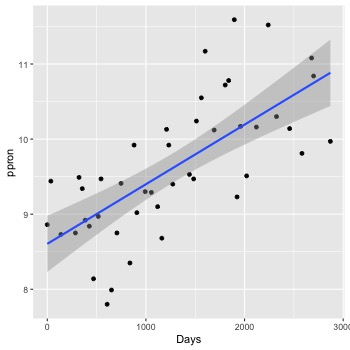
\includegraphics[width=150px, height=150px,  natwidth=300, natheight=300]{RRppronLM.jpg}
		\caption{RR Personal Pronouns - Linear Model}
	\end{minipage}		
	
	\begin{minipage}[b]{0.4\textwidth}
		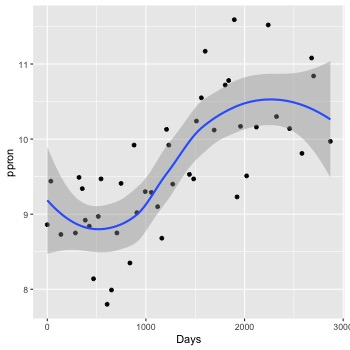
\includegraphics[width=150px, height=150px, natwidth=300, natheight=300]{RRppronLOESS.jpg}
		\caption{RR Personal Pronouns - Local Regression Model}
	\end{minipage}		
\end{figure}
 
There are limitations of this research. Whilst in terms of age, DJT is certainly more suitable as a control to match with RR, in some ways they held very different styles of press conferences in that RR preferred to do solo press conferences and DJT has shown a preference for doing joint press conferences which have an impact on the amount of language produced. This artifact of the data is in itself notable as it illustrates the problems we may have with smaller amounts of speech. Also, the problem of finding an appropriate control is a common one in this domain. Given that those with MCI and early dementia have such variable presentations, it might prove of limited value in matched pairs design. 
\par 
With further work, it is not feasible to the vast array of samples over a timeframe, as we have had with the president corpus and so it would be worth exploring how the quality of these predictions might lessen when faced with considerably fewer samples and over a smaller time period. It would also be worth extending this research further to encompass more of the linguistic features Fraser used in her work \cite{Fraser2015} to see if there are any further insights to be gained. In addition, this replication and extension has demonstrated the potential utility of using longitudinal data as a means of comparing language use of a person at two or more time periods and using this information as a diagnostic aid for MCI and therefore more work would be helpful from a longitudinal perspective to see if this approach may be valid in moving towards a solution for this particular problem. 

\section{Conclusions}\label{conclusions}
The results of this work show that we can track a person's use of language through time in a number of ways, and it is possible for an individual to be his or her own control. This is important as it means the heterogenous nature of the MCI population does not impact results as much as if we were comparing those with MCI to controls. Equally, it would be helpful to have controls to ascertain what would be usual to expect in the decline of language in a healthy older adult. 

\bibliographystyle{apalike}
\bibliography{main3}

\end{document}
